% =============================================================================
%  Subsection: Resource and Cost
%              OIDC-Only, Private-key DID/VC, zkLogin-Only, Action-EHR,
%              zkEHR, zkDIDProof.
%
%  Drop-in for the experiment / analysis section of the zkEHR paper.
%
%  Required preamble (in the main paper):
%    \usepackage{booktabs}
%    \usepackage{graphicx}
%    \usepackage{amsmath}
%    \usepackage{multirow}
%
%  Required figure files (next to this .tex, or anywhere on \graphicspath):
%    storage-comparison.pdf
%    communication-comparison.pdf
%    gas-comparison.pdf
%    resource-and-cost.pdf       (3-panel composite, optional alternative)
%  All produced by make_figure.py.
% =============================================================================

\subsection{Resource and Cost}
\label{ssub:resource-and-cost}

We characterise the deployment cost of each scheme along three axes:
how many bytes each party must keep durably (\emph{storage}), how many
bytes flow on the wire per interaction (\emph{communication}), and how
much chain gas the on-chain operations consume (\emph{gas}). The three
axes are not independent: on-chain object sizes propagate from storage
into communication (when those objects are read or written) and into gas
(via Sui's per-byte storage coefficient). Sizes are derived theoretically
from the Move struct definitions, the TypeScript type schemas, and the
serialized JSON fixtures of the six sibling experiment trees; gas is
estimated from Sui's published gas-cost coefficients applied to those same
on-chain object sizes. No run-time measurement is involved.\footnote{We
report on-the-wire bytes (BCS for chain artefacts, JSON for off-chain
artefacts) at the canonical message granularity of each scheme, durable
state that remains after a flow finishes (transient artefacts excluded),
and the creation-cost component of gas (storage rebate on object deletion
is not credited). Globally amortised state---OIDC JWKS caches, the
Groth16 verification key, salt-authority seeds, institutional ES256
keypairs---is excluded throughout so the comparison reflects \emph{marginal}
cost per additional patient or interaction.}

The six schemes split along three structural axes that determine almost
all of their resource budgets: (i)~whether identity material is anchored
on chain (Action-EHR, Private-DID/VC, and \textsf{zkEHR} yes; the other
three no); (ii)~whether a Groth16 proof rides each interaction
(zkLogin-Only, \textsf{zkEHR}, \textsf{zkDIDProof} yes); and (iii)~whether
the verifier must issue an on-chain RPC at presentation time
(Private-DID/VC, Action-EHR, and \textsf{zkEHR} yes; \textsf{zkDIDProof}
no, \emph{by design}). Storage, communication, and gas costs all fall
out of these three switches.

% -----------------------------------------------------------------------------
% STORAGE
% -----------------------------------------------------------------------------
\paragraph{Storage.}
Table~\ref{tab:storage-comparison} and
Figure~\ref{fig:storage-comparison} expose three regimes.
\textsf{OIDC-Only} and \textsf{zkDIDProof} are the two zero-on-chain
schemes: they keep relying-party state to a single in-memory session
record ($\sim\!300$--$500\,\mathrm{B}$). \textsf{zkDIDProof} drives the
patient cost down to a single field element. The DID is \emph{derived
in-circuit} from
$\mathrm{Poseidon}(\mathrm{sub},\,\mathrm{iss},\,\mathrm{salt})$, so it
need never be materialised as a private key or anchored on chain; in
practice, however, the patient's wallet caches the resulting 32-byte
field element so that subsequent sessions skip the Poseidon recomputation
and the wallet can display a stable identifier to the user. The cache
holds no authority over the identity---it can be deleted and rebuilt
from the OIDC subject, the issuer, and the salt at any time---so the
durable patient footprint is still the smallest of any scheme by an
order of magnitude.
\textsf{Action-EHR} and \textsf{zkLogin-Only} occupy a middle regime in
which the patient holds a small private key and the chain holds a
per-grant access object ($\sim\!400\,\mathrm{B}$).
\textsf{Private-key DID/VC} and \textsf{zkEHR} occupy the high regime,
but for different reasons. \textsf{Private-DID/VC} pays for an on-chain
DID document ($\sim\!575\,\mathrm{B}$) and a long-term private key plus
the held credential at the patient ($\sim\!750\,\mathrm{B}$).
\textsf{zkEHR} shifts the cost to the chain ($\sim\!650\,\mathrm{B}$ for
a DID object plus $\sim\!400\,\mathrm{B}$ per access grant) and keeps
the issuer's mandatory per-patient state to a small \emph{signed
profile} ($\sim\!600\,\mathrm{B}$)---a record of fields such as display
name, role tags, and the institution's signature, keyed by the patient's
DID. Critically, this profile is format-agnostic: it can be a plain
JSON record, a JWT-signed claim set, or any other attestation the
institution prefers, and is the same kind of data an OIDC issuer such as
Google already maintains. \textsf{zkEHR} does \emph{not} require the
issuer to materialise the profile as a W3C verifiable credential; doing
so is an \emph{optional} extension that adds $\sim\!12\,\mathrm{KB}$ per
credential and only earns its keep when selective disclosure or
holder-presentable artefacts are actually wanted. These durable
footprints become wire bytes whenever an object is created, read, or
transmitted, which the next paragraph quantifies.

% -----------------------------------------------------------------------------
% Per-party storage table
% -----------------------------------------------------------------------------
\begin{table}[t]
  \centering
  \small
  \caption{Durable storage per patient, per party. Bytes are mid-range
    estimates derived from the on-chain Move structs and off-chain JSON
    schemas of the six experiment trees; transient state and globally
    amortised state are excluded. Hospital A is the issuer/data holder;
    Hospital B is the cross-institution verifier. ``--'' denotes a party
    that the scheme does not model. Smaller is better.}
  \label{tab:storage-comparison}
  \begin{tabular}{lrrrr}
    \toprule
                                  & Patient & Hosp.\ A          & Hosp.\ B           & On-chain \\
    \midrule
    OIDC-Only                     & $0$           & $\sim\!500$       & --                 & $0$        \\
    Private-key DID/VC            & $\sim\!750$   & $\sim\!64$        & $0^{\dagger}$      & $\sim\!575$ \\
    zkLogin-Only                  & $\sim\!230$   & $\sim\!300$       & --                 & $\sim\!450$ \\
    Action-EHR                    & $\sim\!350$   & $\sim\!50$        & $0^{\dagger}$      & $\sim\!400$ \\
    \textbf{zkEHR (ours)}         & $\sim\!50$    & $\sim\!600^{\S}$  & $0^{\dagger}$      & $\sim\!650$ \\
    \textbf{zkDIDProof (ours)}    & $\mathbf{\sim\!32^{\ddagger}}$ & $\sim\!300$ & --       & $\mathbf{0}$ \\
    \bottomrule
  \end{tabular}
  \par\medskip
  {\footnotesize $^{\dagger}$\,Verifier holds a transient cache only; no
    durable per-patient row.\\
    $^{\ddagger}$\,The patient's wallet caches one field element---the
    DID $=\mathrm{Poseidon}(\mathrm{sub},\,\mathrm{iss},\,\mathrm{salt})$,
    32\,B---to avoid recomputing it each session.\\
    $^{\S}$\,Mandatory issuer state only: a profile keyed by the
    patient's DID and signed by the institution's key, in any format.
    Issuing a W3C verifiable credential is an \emph{optional} extension
    that would add $\sim\!12\,\mathrm{KB}$ per credential.}
\end{table}

\begin{figure}[t]
  \centering
  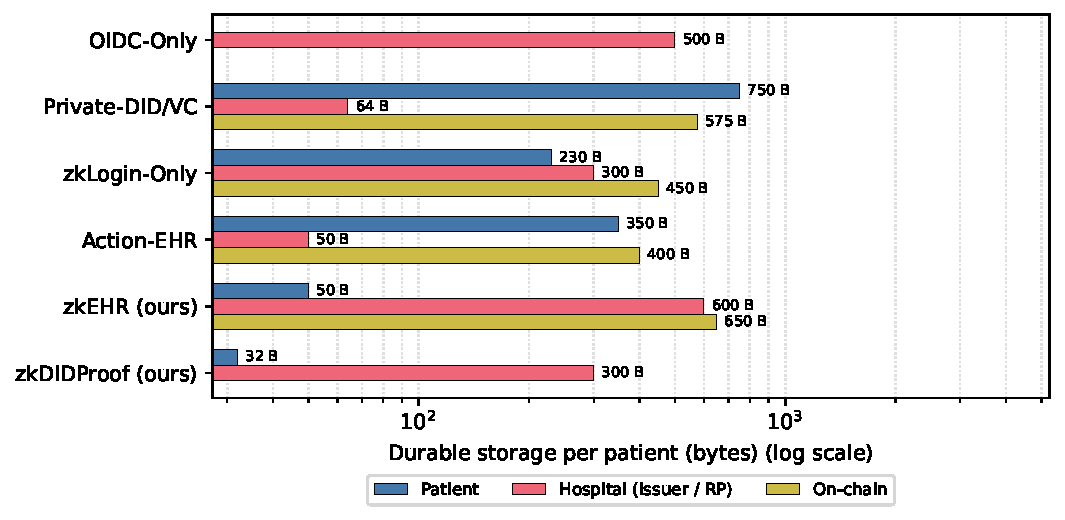
\includegraphics[width=\columnwidth]{storage-comparison}
  \caption{Durable per-patient storage by scheme, broken down by party.
    Bars are drawn on a log scale; missing bars denote zero-byte cells.
    The \textsf{zkEHR} issuer bar shows only the \emph{mandatory}
    per-patient state. \textsf{zkDIDProof} is the only scheme with zero
    on-chain state and a patient footprint of just one cached field
    element ($32\,\mathrm{B}$ DID).}
  \label{fig:storage-comparison}
\end{figure}

% -----------------------------------------------------------------------------
% COMMUNICATION
% -----------------------------------------------------------------------------
\paragraph{Communication.}
Table~\ref{tab:communication-comparison} and
Figure~\ref{fig:communication-comparison} make the bandwidth profile of
each scheme explicit. Three schemes---\textsf{OIDC-Only},
\textsf{zkLogin-Only}, and \textsf{zkDIDProof}---share the same OIDC
primitive against Google (authorisation URL $\to$ code callback $\to$
token POST $\to$ JWT response), each round-trip costing a recurrent
$\sim\!3$--$4\,\mathrm{KB}$ and adding a one-time JWKS fetch of
$\sim\!2$--$5\,\mathrm{KB}$ on cold starts. The three schemes differ
only in the OAuth profile they use (Authorisation Code with PKCE in
\textsf{OIDC-Only} and \textsf{zkDIDProof}; Implicit flow in
\textsf{zkLogin-Only}) and in what nonce is bound into the JWT---a
verifier challenge in \textsf{zkDIDProof}, a hash of the ephemeral
public key plus maximum-epoch in \textsf{zkLogin-Only}, no
cryptographic binding in \textsf{OIDC-Only}. Their headline
establishment / presentation totals diverge because of what they
\emph{add on top} of the shared primitive.
\textsf{Action-EHR} has \emph{no} establishment phase at all---the
patient signs an access grant directly with a long-term key---and its
only on-the-wire cost is the cross-institution access call
($\sim\!3.5\,\mathrm{KB}$, dominated by the Sui transaction envelope and
the \texttt{getObject} response). \textsf{zkDIDProof} sits at the
symmetric opposite: there is no establishment, no chain RPC at
presentation, and a single $\sim\!4.3\,\mathrm{KB}$ presentation bundle
(an OIDC round-trip $\sim\!3.4\,\mathrm{KB}$ plus a proof-and-signals
bundle of $\sim\!600\,\mathrm{B}$, broken down below) carries the entire
protocol. \textsf{zkLogin-Only} ($\sim\!8\,\mathrm{KB}$ establishment)
layers a salt-service round-trip ($\sim\!1.5\,\mathrm{KB}$ up,
$\sim\!0.1\,\mathrm{KB}$ down) and a Mysten-prover round-trip
($\sim\!1.7\,\mathrm{KB}$ up, $\sim\!0.4\,\mathrm{KB}$ down) on top of
the OIDC primitive, then submits a Sui transaction with the inflated
zkLogin signature ($\sim\!2\,\mathrm{KB}$). \textsf{zkEHR} has the
heaviest establishment of any scheme ($\sim\!12.4\,\mathrm{KB}$ for
$N=3$ salt authorities) because it fans out the salt request to $N$
authorities at $\sim\!1.45\,\mathrm{KB}$ each and then registers a DID
object on chain; in return its per-access cost ($\sim\!1.9\,\mathrm{KB}$)
is competitive with the cheapest chain-using baseline.
For the four chain-using schemes, the on-chain bytes additionally
translate into Sui storage fees through the protocol's per-byte
coefficient and the per-transaction computation cost, which the next
paragraph quantifies.

\paragraph{The $\sim\!600\,\mathrm{B}$ presentation bundle.}
The bundle that \textsf{zkDIDProof} sends to the verifier consists of
the Groth16 proof and the four public signals against which the proof
is checked. The proof itself,
$\pi=(\pi_A,\pi_B,\pi_C)$ with $\pi_A,\pi_C\in G_1$ and $\pi_B\in G_2$
on the BN128 curve, is $\sim\!256\,\mathrm{B}$ when serialised by
\texttt{snarkjs} as compressed-coordinate JSON. The public signals are
four BN128 scalar-field elements rendered as decimal strings
($\sim\!78$ characters each, $\sim\!312\,\mathrm{B}$ total): the
patient's
\textsf{DID}~$=\mathrm{Poseidon}(\mathrm{sub},\,\mathrm{iss},\,
\mathrm{salt})$, the audience binding \textsf{aud}, an expiry anchor
$T_{\mathrm{exp}}$, and the verifier-issued challenge \textsf{chal} that
forces freshness. These four signals are exactly what the verifier
needs to relate the proof back to the relying party's local state
without ever looking at the JWT itself or contacting a chain. The total
$\sim\!568\,\mathrm{B}$ rounds to the $\sim\!600\,\mathrm{B}$ row in the
table.

% -----------------------------------------------------------------------------
% Per-interaction communication table
% -----------------------------------------------------------------------------
\begin{table}[t]
  \centering
  \small
  \caption{Communication per interaction (wire bytes). Establishment is
    the one-shot identity / DID creation flow; per-presentation is one
    credential presentation to a relying party; cross-institution access
    is one access query from Hospital B against an on-chain grant or
    off-chain consent. ``--'' indicates the scheme has no separate phase
    of that type. Smaller is better.}
  \label{tab:communication-comparison}
  \begin{tabular}{lrrr}
    \toprule
                                  & Establishment & Presentation & Cross-inst.\ access \\
    \midrule
    OIDC-Only                     & $7{,}500$    & $1{,}500$        & $1{,}100$           \\
    Private-key DID/VC            & $1{,}200$    & $\phantom{0}800$ & $1{,}200$           \\
    zkLogin-Only                  & $8{,}000$    & --               & $1{,}100$           \\
    Action-EHR                    & --           & --               & $3{,}500$           \\
    \textbf{zkEHR (ours)}         & $12{,}400$   & --               & $1{,}900$           \\
    \textbf{zkDIDProof (ours)}    & --           & $4{,}300$        & --                  \\
    \bottomrule
  \end{tabular}
\end{table}

\begin{figure}[t]
  \centering
  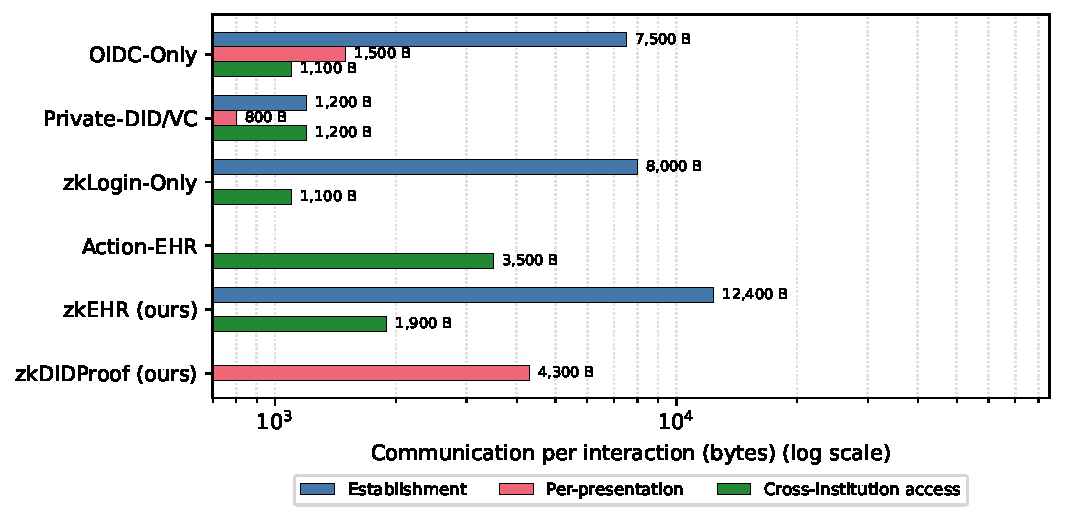
\includegraphics[width=\columnwidth]{communication-comparison}
  \caption{Wire bytes per interaction by scheme, decomposed into the
    establishment phase, the per-presentation bundle, and the
    cross-institution access query. Bars are drawn on a log scale.
    \textsf{zkEHR} pays the largest establishment cost (multi-authority
    salt fan-out at $N\!=\!3$) and the smallest per-access cost among
    chain-using schemes; \textsf{zkDIDProof} folds the entire protocol
    into a single $\sim\!4.3\,\mathrm{KB}$ presentation with no
    establishment phase and no chain RPC.}
  \label{fig:communication-comparison}
\end{figure}

% -----------------------------------------------------------------------------
% GAS
% -----------------------------------------------------------------------------
\paragraph{Gas.}
Table~\ref{tab:gas-comparison} and Figure~\ref{fig:gas-comparison} price
the on-chain operations of each scheme using Sui's documented gas
formula
$\text{gas} = g_{\text{tx}} + c_{\text{store}}\!\cdot\!|\text{object}|$,
where $g_{\text{tx}}$ is the per-transaction computation cost and
$c_{\text{store}}\!\approx\!100\,\mathrm{MIST}/\mathrm{B}$ is Sui's
per-byte storage coefficient.\footnote{Sui's storage rebate on object
deletion (${\approx}99\%$ of $c_{\text{store}}\!\cdot\!|\text{object}|$)
is excluded because we are pricing object \emph{creation}; objects
remain live in our analysis.} The two cryptographic regimes diverge
sharply on $g_{\text{tx}}$: an Ed25519-signed transaction baseline costs
roughly $g_{\text{tx}}^{\text{ed}}\!\approx\!8\!\times\!10^{5}\,\mathrm{MIST}$,
whereas a zkLogin-signed transaction additionally pays for an on-chain
Groth16 verification, raising it to
$g_{\text{tx}}^{\text{zk}}\!\approx\!1.5\!\times\!10^{6}\,\mathrm{MIST}$.
The four chain-using schemes split into two tiers along this line.
\textsf{Private-DID/VC} and \textsf{Action-EHR}, both Ed25519-signed,
pay $\sim\!0.86\!\times\!10^{6}\,\mathrm{MIST}$ for one DID-object
registration and $\sim\!0.84\!\times\!10^{6}\,\mathrm{MIST}$ per access
grant respectively. \textsf{zkLogin-Only} and \textsf{zkEHR}, both
zkLogin-signed at the patient, pay
$\sim\!1.55\!\times\!10^{6}\,\mathrm{MIST}$ per chain interaction. Two
schemes contribute zero gas on every axis: \textsf{OIDC-Only} (no chain
interaction) and \textsf{zkDIDProof} (verifier-side proof verification
is local). The asymmetry in the table is therefore a direct read-out
of which schemes anchor identity on chain and what kind of signature
they use to do so.

% -----------------------------------------------------------------------------
% Per-interaction gas table
% -----------------------------------------------------------------------------
\begin{table}[t]
  \centering
  \small
  \caption{On-chain gas per interaction (MIST), theoretical, derived from
    Sui's gas-cost coefficients applied to the on-chain object sizes of
    Table~\ref{tab:storage-comparison}. Establishment is the one-shot
    identity / DID creation flow; per-access is one cross-institution
    grant transaction. Per-presentation gas is zero for every scheme
    (presentation reads are RPC \texttt{getObject} calls, which are
    free) and is omitted. ``$0$'' means the scheme has no chain
    interaction in that phase. Smaller is better.}
  \label{tab:gas-comparison}
  \begin{tabular}{lrr}
    \toprule
                                  & Establishment           & Per-access \\
    \midrule
    OIDC-Only                     & $0$                     & $0$ \\
    Private-key DID/VC            & $\sim\!860{,}000$       & $0$ \\
    zkLogin-Only                  & $\sim\!1{,}550{,}000$   & $\sim\!1{,}550{,}000$ \\
    Action-EHR                    & $0$                     & $\sim\!840{,}000$ \\
    \textbf{zkEHR (ours)}         & $\sim\!1{,}570{,}000$   & $\sim\!1{,}540{,}000$ \\
    \textbf{zkDIDProof (ours)}    & $\mathbf{0}$            & $\mathbf{0}$ \\
    \bottomrule
  \end{tabular}
\end{table}

\begin{figure}[t]
  \centering
  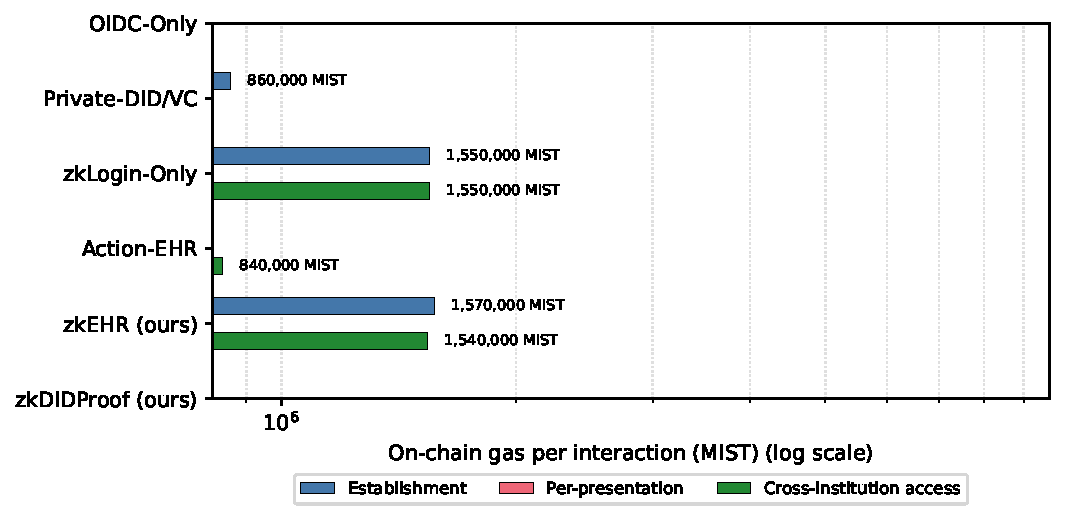
\includegraphics[width=\columnwidth]{gas-comparison}
  \caption{On-chain gas per interaction by scheme, in MIST. Bars are
    drawn on a log scale; missing bars denote schemes with no chain
    interaction in that phase. The two zk-signed schemes
    (\textsf{zkLogin-Only}, \textsf{zkEHR}) form the upper tier at
    $\sim\!1.55\!\times\!10^{6}\,\mathrm{MIST}$ per chain interaction;
    the two Ed25519-signed schemes (\textsf{Private-DID/VC},
    \textsf{Action-EHR}) form the lower tier at
    $\sim\!0.85\!\times\!10^{6}\,\mathrm{MIST}$. \textsf{OIDC-Only} and
    \textsf{zkDIDProof} are absent from the figure because both pay
    zero gas on every axis.}
  \label{fig:gas-comparison}
\end{figure}

% -----------------------------------------------------------------------------
% UNIFIED CLOSED-FORM MODELS
% -----------------------------------------------------------------------------
\paragraph{Closed-form cost models.}
The same variables drive all three axes. Let $J\!\approx\!1.3\,\mathrm{KB}$
be the size of a Google ID token, $\pi\!\approx\!0.3\,\mathrm{KB}$ a
Groth16 proof, $T\!\approx\!1.4\,\mathrm{KB}$ a Sui transaction
envelope, $S\!\approx\!0.15\,\mathrm{KB}$ a single-authority salt
response, $P\!\approx\!0.6\,\mathrm{KB}$ a signed issuer profile,
$V\!\approx\!12\,\mathrm{KB}$ an \emph{optional} W3C verifiable
credential, $\sigma\!\approx\!64\,\mathrm{B}$ an Ed25519 signature,
$O_{\text{did}}\!\approx\!0.5\,\mathrm{KB}$ a chain DID object,
$O_{\text{grant}}\!\approx\!0.4\,\mathrm{KB}$ a chain access grant,
$g_{\text{tx}}^{\text{ed}}\!\approx\!8\!\times\!10^{5}\,\mathrm{MIST}$
and
$g_{\text{tx}}^{\text{zk}}\!\approx\!1.5\!\times\!10^{6}\,\mathrm{MIST}$
the per-transaction computation costs for the two signature regimes,
$c_{\text{store}}\!\approx\!100\,\mathrm{MIST}/\mathrm{B}$ Sui's per-byte
storage coefficient, $N$ the number of salt authorities, and $G$ the
number of grants per patient. The asymptotic costs are then:
\begin{align*}
  \text{OIDC-Only:}\quad        & \mathcal{S}_{\text{issuer}} \!\approx\! P,\;\;
                                  \mathcal{C}_{\text{est}} \!\approx\! 2J,\;\;
                                  \mathcal{G} \!=\! 0\,, \\
  \text{Private-DID/VC:}\quad   & \mathcal{S}_{\text{patient}} \!\approx\! V\!+\!O_{\text{did}},\;\;
                                  \mathcal{C}_{\text{pres}} \!\approx\! V\!+\!\sigma,\;\;
                                  \mathcal{G}_{\text{est}} \!\approx\! g_{\text{tx}}^{\text{ed}}\!+\!c_{\text{store}}O_{\text{did}}\,, \\
  \text{zkLogin-Only:}\quad     & \mathcal{S}_{\text{chain}} \!\approx\! G\!\cdot\!O_{\text{grant}},\;\;
                                  \mathcal{C}_{\text{est}} \!\approx\! J\!+\!S\!+\!\pi\!+\!T,\;\;
                                  \mathcal{G}_{\text{est}} \!\approx\! g_{\text{tx}}^{\text{zk}}\!+\!c_{\text{store}}O_{\text{grant}}\,, \\
  \text{Action-EHR:}\quad       & \mathcal{S}_{\text{chain}} \!\approx\! G\!\cdot\!O_{\text{grant}},\;\;
                                  \mathcal{C}_{\text{acc}} \!\approx\! 2T,\;\;
                                  \mathcal{G}_{\text{acc}} \!\approx\! g_{\text{tx}}^{\text{ed}}\!+\!c_{\text{store}}O_{\text{grant}}\,, \\
  \text{\textsf{zkEHR}:}\quad   & \mathcal{S}_{\text{chain}} \!\approx\! O_{\text{did}}\!+\!G\!\cdot\!O_{\text{grant}},\;\;
                                  \mathcal{C}_{\text{est}} \!\approx\! J\!+\!N\!\cdot\!S\!+\!\pi\!+\!T,\;\;
                                  \mathcal{G}_{\text{est}} \!\approx\! g_{\text{tx}}^{\text{zk}}\!+\!c_{\text{store}}O_{\text{did}}\,, \\
  \text{\textsf{zkDIDProof}:}\quad & \mathcal{S}_{\text{chain}} \!=\! 0,\;\;
                                  \mathcal{C}_{\text{pres}} \!\approx\! J\!+\!\pi,\;\;
                                  \mathcal{G} \!=\! 0\,.
\end{align*}
Three structural observations follow from reading the same variables
across the three axes. First, the on-chain object sizes
$O_{\text{did}}$ and $O_{\text{grant}}$ appear in both
$\mathcal{S}_{\text{chain}}$ and $\mathcal{G}$: gas grows linearly in
exactly the same bytes that storage does, with $c_{\text{store}}$ as
the conversion constant. Second, \textsf{zkEHR}'s communication cost is
the only one that grows linearly in $N$ (the number of salt
authorities); this $N\!\cdot\!S$ tail buys decentralised trust over the
keyless-recovery seed, and is paid in bytes only---it does \emph{not}
appear in the gas axis, because the salt service is off-chain. Third,
\textsf{zkDIDProof} is the only scheme whose chain storage and chain
gas are simultaneously identically zero; the relying party retains only
a verification key amortised over its entire user population.

% -----------------------------------------------------------------------------
% TAKE-AWAY
% -----------------------------------------------------------------------------
\paragraph{Take-away.}
Reading the three axes together rather than in isolation reveals
patterns no single axis can show. \textsf{zkDIDProof} minimises all
three axes simultaneously by removing every chain interaction; it pays
its costs in patient-side proving time (Section~\ref{ssub:presentation-latency})
rather than on chain. \textsf{zkEHR} pays modestly on every axis and is
the only scheme whose multi-authority salt cost grows with $N$
($N\!\cdot\!S$), visible on the communication axis but \emph{invisible}
on the gas axis because the salt service is off-chain. \textsf{Action-EHR}
has zero communication establishment but pays per-grant on storage,
communication, and gas simultaneously---the only scheme to do so.
\textsf{Private-DID/VC} is dominated by the held VC: $V$ governs both
patient storage and per-presentation communication, but does not touch
gas after one-time DID registration. \textsf{zkLogin-Only} is the
mirror of \textsf{Action-EHR}: heavy establishment communication but
relatively cheap per-grant traffic, with gas in the upper tier because
of the on-chain Groth16 verification. \textsf{OIDC-Only} is the
absolute baseline: lightest on every axis, but provides neither
decentralised identity nor offline verifiability. The three figures
and three tables in this subsection thus locate every scheme on the
same resource plane, and together with the latency analysis of
Section~\ref{ssub:presentation-latency} they characterise the full
deployment cost of each design.
